\section{Auswertung}
\label{sec:Auswertung}

\subsection{Bragg-Bedingung}
\label{sec:Bragg}

Die Messwerte zur Überprüfung der Bragg-Bedingung sind in \autoref{tab:Bragg} zu finden und in \autoref{fig:bragg}
dargestellt. Es wurde ein Maxium bei $27,7^{\circ}$ festgestellt. Nachdem Reflexionsgesetz liegt der
theoretische Winkel bei $28^{\circ}$. Daraus ergibt sich eine Abweichung von $1,5\%$.

\begin{table}
  \centering
  \begin{tabular}{c c | c c}
    \toprule
    $\theta^{\circ}$ & $N/Imp/s$ & $\theta^{\circ}$ & $N/Imp/s$ \\
    \midrule
    26,0 &  39,0 & 28,2 & 272,0 \\
    26,1 &  43,0 & 28,3 & 263,0 \\
    26,2 &  43,0 & 28,4 & 255,0 \\
    26,3 &  52,0 & 28,5 & 247,0 \\
    26,4 &  76,0 & 28,6 & 234,0 \\
    26,5 &  85,0 & 28,7 & 236,0 \\
    26,6 & 113,0 & 28,8 & 222,0 \\
    26,7 & 117,0 & 28,9 & 206,0 \\
    26,8 & 146,0 & 29,0 & 181,0 \\
    26,9 & 164,0 & 29,1 & 185,0 \\
    27,0 & 183,0 & 29,2 & 164,0 \\
    27,1 & 182,0 & 29,3 & 155,0 \\
    27,2 & 216,0 & 29,4 & 154,0 \\
    27,3 & 219,0 & 29,5 & 129,0 \\
    27,4 & 238,0 & 29,6 & 110,0 \\
    27,5 & 256,0 & 29,7 & 100,0 \\
    27,6 & 281,0 & 29,8 &  90,0 \\
    27,7 & 277,0 & 29,9 &  84,0 \\
    27,8 & 274,0 & 30,0 &  75,0 \\
    27,9 & 269,0 & & \\
    28,0 & 278,0 & & \\
    28,1 & 274,0 & & \\
    \bottomrule
  \end{tabular}
  \caption{Messwerte zur Überrüfung der Bragg-Bedingung.}
  \label{tab:Bragg}
\end{table}

\begin{figure}
  \centering
  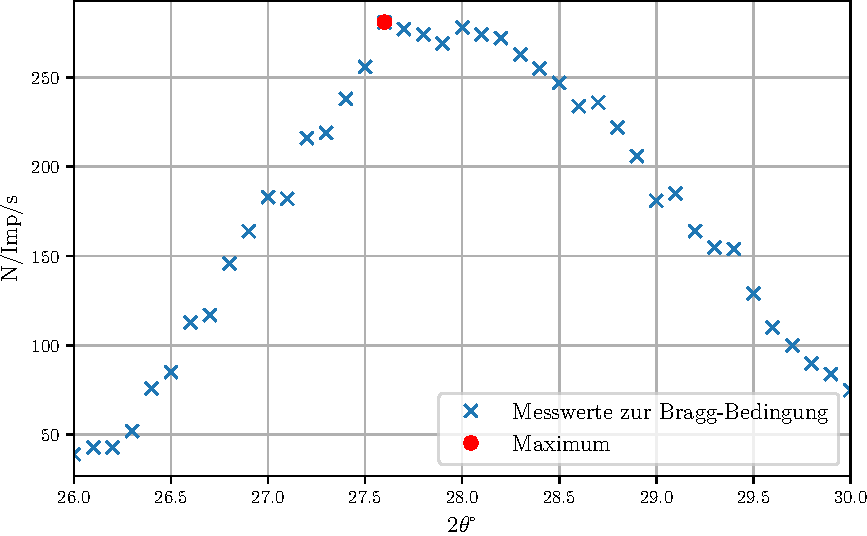
\includegraphics{bragg.pdf}
  \caption{Werte zur Bestimmung der Bragg-Bedingung.}
  \label{fig:bragg}
\end{figure}

\subsection{Emissionsspektrum der Cu-Röntgenröhre}
\label{sec:cu}

\begin{figure}
  \centering
  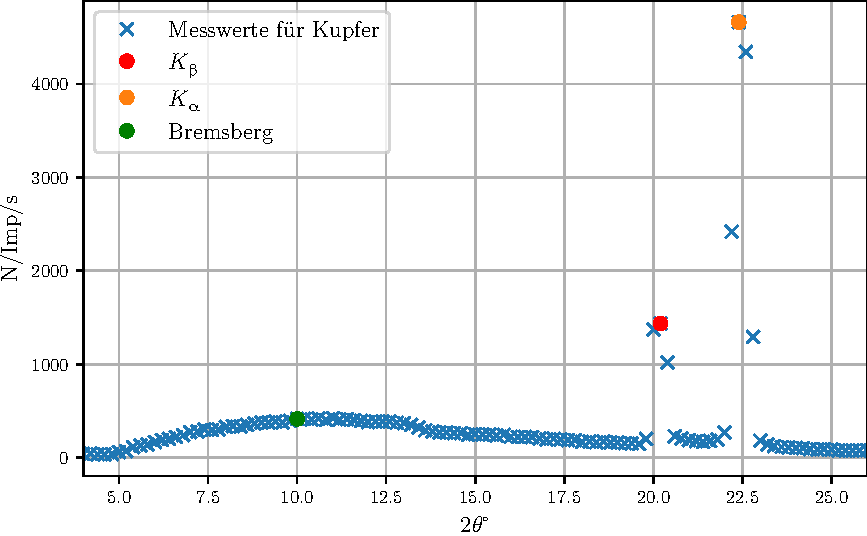
\includegraphics{cu.pdf}
  \caption{Emissionsspektrum der Cu-Röntgenröhre.}
  \label{fig:cu}
\end{figure}